\documentclass{beamer}

\usepackage{graphicx}

\usepackage[utf8]{inputenc}

\usepackage{natbib}
\usepackage{textcomp}
\usepackage[greek,english]{babel}
\usepackage{amsmath}

\usepackage{physics}

\usefonttheme[onlymath]{serif}
\setbeamertemplate{footline}[frame number]

\frenchspacing
%\renewcommand{\thefootnote}{\alph{footnote}}

\begingroup
\lccode`\~=`\ %
\lowercase{%
  \gdef\assignment{\setcounter{word}{0}%
    \catcode`~=\active
    \def~{\space\stepcounter{word}}}}%
\endgroup
\newcounter{word}
\def\endassignment{\stepcounter{word}%
  \begin{flushright}%
  (\arabic{word} words)%
  \end{flushright}%
}

\title{Still water and other hard-to-model systems}

\author{Martin Büttner \\ {\footnotesize Supervisor: Prof. Ted Johnson}}
\date{16 March, 2015}

\begin{document}

\frame{\titlepage}

\begin{frame}
  \frametitle{The Shallow Water Equations}
  \begin{itemize}
    \item Simplified fluid model:
    \begin{itemize}
      \item Incompressible
      \item Inviscid
      \item \emph{Shallow} (horizontal length scale $\gg$ typical depth)
    \end{itemize}
    \item Used to model oceans \only<2->{($\sim$ 4km deep)} \\
          and atmosphere \only<2->{($\sim$ 10km deep)}
  \end{itemize}
  \pause\pause
  \begin{align}
                           h_t + (hu)_x & = 0 \\
    (hu)_t + \qty(hu^2 + \frac{1}{2}gh^2)_x & = 0 \\
                       (hv)_t + (huv)_x & = 0
  \end{align}
\end{frame}

\begin{frame}
  \frametitle{Finite Volume Methods}
  \begin{itemize}
    \item Developed for \emph{hyperbolic conservation laws}:
    \begin{equation}
      \vb q_t + \vb f(\vb q)_x = 0
    \end{equation}
    \item Discretisation:\\ \vspace{0.2cm}
    \begin{center}
      \includegraphics<1>[width=0.5\textwidth]{img/discr1}
      \includegraphics<2>[width=0.5\textwidth]{img/discr2}
      \includegraphics<3>[width=0.5\textwidth]{img/discr3}
      \includegraphics<4>[width=0.5\textwidth]{img/discr4}
  \end{center}
  \end{itemize}
\end{frame}

\begin{frame}
  \frametitle{Riemann Problems}
  \begin{center}
    \includegraphics<1>[width=0.9\textwidth]{img/riemann1}
    \includegraphics<2->[width=0.9\textwidth]{img/riemann2}
  \end{center}
  \begin{itemize}
    \item Initial value problem: step function
    \item<2-> Decompose into waves
    \item<3-> Finite speeds $\Rightarrow$ only affect neighbouring cells
  \end{itemize}
\end{frame}

\begin{frame}
  \frametitle{Godunov's Method}
  \begin{itemize}
    \item Wave propagation form:
      \begin{equation}
        Q_i^{n+1} = Q_i^n - \frac{\Delta t}{\Delta x} (\mathcal{A}^+ \Delta Q_{i-1/2} + \mathcal{A}^- \Delta Q_{i+1/2})
      \end{equation}
      \pause
      \begin{align}
        \mathcal{A}^- \Delta Q_{i-1/2} &= \sum_{p=1}^{M_w} (s_{i-1/2}^p)^-\mathcal{W}_{i-1/2}^p \\
        \mathcal{A}^+ \Delta Q_{i+1/2} &= \sum_{p=1}^{M_w} (s_{i+1/2}^p)^+\mathcal{W}_{i+1/2}^p
      \end{align}
  \end{itemize}
\end{frame}

\begin{frame}
  \frametitle{Implementation: Clawpack}
  \begin{itemize}
    \item ``\textbf{C}onservation \textbf{law} \textbf{pack}age'', by Randall J. LeVeque, 1994
    \pause
    \item Riemann solvers in Fortran 90
    \begin{itemize}
      \item Take grid data, compute wave decomposition
    \end{itemize}
    \pause
    \item Configuration in Python 2
    \begin{itemize}
      \item Grid setup
      \item Initial conditions
      \item Boundary conditions
      \item Plotting instructions
    \end{itemize}
  \end{itemize}
\end{frame}

\begin{frame}
  \frametitle{Adding Source Terms}
  \begin{itemize}
  \item Modelling additional effects:
  \begin{align}
                           h_t + (hu)_x & = 0 \hspace{0.25\textwidth}\\
    (hu)_t + \qty(hu^2 + \frac{1}{2}gh^2)_x & = \alt<3->{-hB_x+Khv}{\alt<2>{-hB_x}{0}} \\
                       (hv)_t + (huv)_x & = \alt<3->{-Khu}{0}
  \end{align}
    \item<4-> Full form of conservation law:
    \begin{equation}
      \vb q_t + \vb f(\vb q)_x = \vb s(\vb q, x)
    \end{equation}
  \end{itemize}
\end{frame}

\begin{frame}[t]
  \frametitle{Adding Source Terms}
  \begin{itemize}
    \item Split into two steps:
    \begin{align}
      \vb q_t + \vb f(\vb q)_x &= 0 \\
      \vb q_t &= \vb s(\vb q, x)
    \end{align}
    \item<2-> The still water system:\\
    \begin{center}
      \includegraphics<2>[width=0.65\textwidth]{img/bathymetry1}
      \includegraphics<3>[width=0.65\textwidth]{img/bathymetry2}
    \end{center}
  \end{itemize}
\end{frame}

\begin{frame}
  \frametitle{Geostrophic Equilibria}
  \begin{itemize}
    \item Coriolis force admits non-trivial equilibria when
    \begin{equation}
      u = 0\qc v = \frac{h (h_s)_x}{K}
    \end{equation}
    \begin{center}
      \raisebox{-0.5\height}{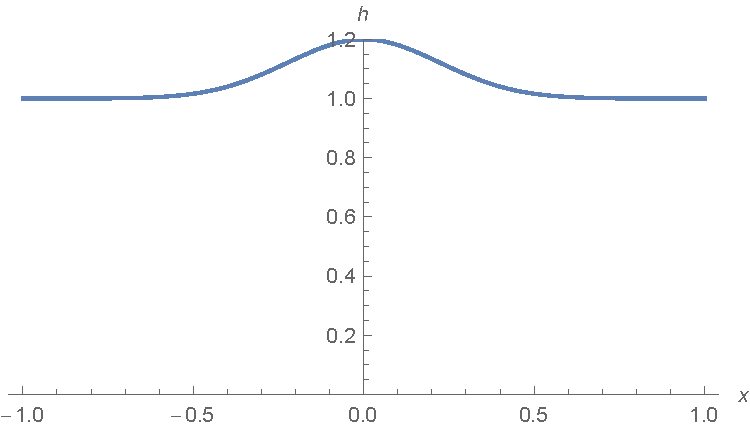
\includegraphics[width=0.45\textwidth]{img/geostrophic-depth}}
      \raisebox{-0.5\height}{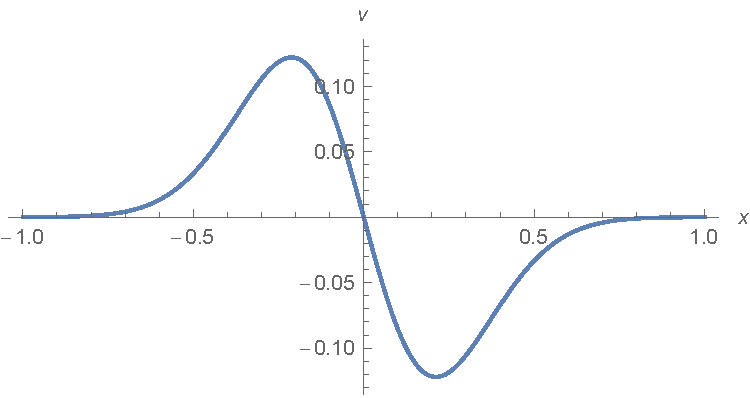
\includegraphics[width=0.45\textwidth]{img/geostrophic-ymom}}
    \end{center}
    \vspace{0.5cm}
    \item Geophysical flows close to geostrophic equilibrium at all times
  \end{itemize}
\end{frame}

\begin{frame}[t]
  \frametitle{Well-Balanced Methods}
  \framesubtitle{LeVeque}
  \begin{itemize}
    \item LeVeque, 1998, ``Balancing Source Terms and Flux Gradients in High-Resolution Godunov Methods: The Quasi-Steady Wave-Propagation Algorithm''
    \vspace{0.5cm}
    \begin{center}
      \includegraphics<2>[width=0.5\textwidth]{img/leveque-splitting1}
      \includegraphics<3->[width=0.5\textwidth]{img/leveque-splitting2}
    \end{center}
    \vspace{0.5cm}
    \only<4>{
      \begin{equation}
        \vb f(Q_i^+) - \vb f(Q_i^-) = \vb s(Q_i, x_i) \Delta x
      \end{equation}
    }
  \end{itemize}
\end{frame}

\begin{frame}
  \frametitle{Well-Balanced Methods}
  \framesubtitle{LeVeque}
  \begin{itemize}
    \item Method originally developed for bathymetry term
    \pause
    \item Derived analogous method including Coriolis terms
    \pause
    \item Pro:
    \begin{itemize}
      \item Well-balanced for all equilibria
    \end{itemize}
    \pause
    \item Con:
    \begin{itemize}
      \item Requires solving cubic for offset
      \item Problematic away from equilibrium (transcritical flow)
    \end{itemize}
  \end{itemize}
\end{frame}

\begin{frame}
  \frametitle{Well-Balanced Methods}
  \framesubtitle{Rogers et al.}
  \begin{itemize}
    \item Rogers, Borthwick, Taylor, 2003, ``Mathematical balancing of flux gradient and source terms prior to using Roe's approximate Riemann solver''
    \pause
    \item Change of variables: deviations from equilibrium
    \begin{align}
      \vb q_t + \vb f(\vb q)_x &= \vb s(\vb q, x) \\
      \to (\vb q - \vb q_\mathrm{eq})_t + (\vb f(\vb q) - \vb f(\vb q_\mathrm{eq}))_x &= \vb s(\vb q, x) - \vb s(\vb q_\mathrm{eq}, x) \\
      \mbox{or} \quad \vb q^*_t + \vb f^*_x &= \vb s^*
    \end{align}
    \pause
    \item At equilibrium, all terms vanish
    \pause
    \item Jacobian of $\vb f$ remains unchanged
    \begin{itemize}
      \item easy to adapt existing solver
    \end{itemize}
  \end{itemize}
\end{frame}

\begin{frame}
  \frametitle{Well-Balanced Methods}
  \framesubtitle{Rogers et al.}
  \begin{itemize}
    \item Derivation in original paper leads to
    \begin{equation}
      \vb q^*_t + \vb f'(\vb q) \vb q^*_x = \vb s^*
    \end{equation}
    \item Implementation based on this failed away from equilibrium
    \pause
    \item Derived alternative form:
    \begin{equation}
      \vb q^*_t + \vb f'(\vb q) \vb q^*_x = \vb s^* - \pdv{\vb f^*}{\vb q_\mathrm{eq}} (\vb q_\mathrm{eq})_x
    \end{equation}
    \item Works, but less accurate than unbalanced method
    \pause
    \item Again, extended original work to support Coriolis term
    \pause
    \item Also derived solver for geostrophic equilibria
    \begin{itemize}
      \item Implementation does not work yet
    \end{itemize}
  \end{itemize}
\end{frame}

\begin{frame}
  \frametitle{Well-Balanced Methods}
  \framesubtitle{Rogers et al.}
  \begin{itemize}
    \item Pro:
    \begin{itemize}
      \item Works away from equilibrium
      \item Fairly simple to derive and implement
    \end{itemize}
    \item Con:
    \begin{itemize}
      \item Tailored to a specific equilibrium
      \item Need to know equilibrium a priori
      \item Less accurate than unbalanced method away from equilibrium
    \end{itemize}
  \end{itemize}
\end{frame}

\begin{frame}
  \frametitle{Evaluation}
  \begin{itemize}
    \item Implemented evaluation framework in Clawpack (Python)
    \item Supports 7 different bathymetries and 5 initial conditions
    \item Implemented 4 Riemann solvers in Fortran (unbalanced, LeVeque, Rogers for still water, Rogers for geostrophic equilibrium)
  \end{itemize}
\end{frame}

\begin{frame}
  \frametitle{Results}
  \framesubtitle{Still water}
  \begin{center}
    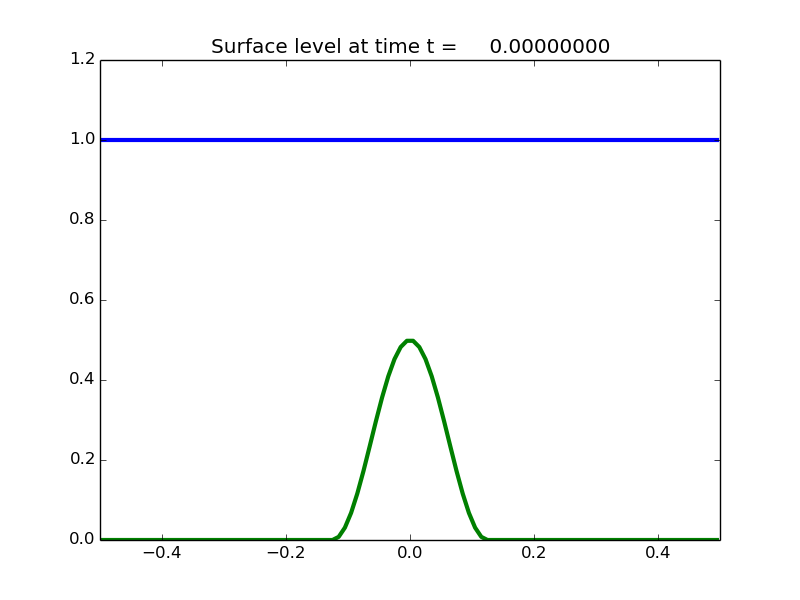
\includegraphics[width=0.45\textwidth]{../results/still-cosine-initial.png}
    \includegraphics<1>[width=0.45\textwidth]{../results/still-cosine-unbalanced-01.png}
    \includegraphics<2>[width=0.45\textwidth]{../results/still-cosine-unbalanced-02.png}
    \includegraphics<3>[width=0.45\textwidth]{../results/still-cosine-unbalanced-03.png}
    \includegraphics<4>[width=0.45\textwidth]{../results/still-cosine-unbalanced-04.png}
    \includegraphics<5>[width=0.45\textwidth]{../results/still-cosine-unbalanced-05.png}
    \includegraphics<6>[width=0.45\textwidth]{../results/still-cosine-unbalanced-06.png}
    \includegraphics<7>[width=0.45\textwidth]{../results/still-cosine-unbalanced-07.png}
    \includegraphics<8>[width=0.45\textwidth]{../results/still-cosine-unbalanced-08.png}
    \includegraphics<9>[width=0.45\textwidth]{../results/still-cosine-unbalanced-09.png}
    \includegraphics<10>[width=0.45\textwidth]{../results/still-cosine-unbalanced-10.png}
    \includegraphics<11>[width=0.45\textwidth]{../results/still-cosine-unbalanced-11.png} \\
    \includegraphics<1>[width=0.45\textwidth]{../results/still-cosine-rogers-01.png}
    \includegraphics<2>[width=0.45\textwidth]{../results/still-cosine-rogers-02.png}
    \includegraphics<3>[width=0.45\textwidth]{../results/still-cosine-rogers-03.png}
    \includegraphics<4>[width=0.45\textwidth]{../results/still-cosine-rogers-04.png}
    \includegraphics<5>[width=0.45\textwidth]{../results/still-cosine-rogers-05.png}
    \includegraphics<6>[width=0.45\textwidth]{../results/still-cosine-rogers-06.png}
    \includegraphics<7>[width=0.45\textwidth]{../results/still-cosine-rogers-07.png}
    \includegraphics<8>[width=0.45\textwidth]{../results/still-cosine-rogers-08.png}
    \includegraphics<9>[width=0.45\textwidth]{../results/still-cosine-rogers-09.png}
    \includegraphics<10>[width=0.45\textwidth]{../results/still-cosine-rogers-10.png}
    \includegraphics<11>[width=0.45\textwidth]{../results/still-cosine-rogers-11.png}
    \includegraphics<1>[width=0.45\textwidth]{../results/still-cosine-leveque-01.png}
    \includegraphics<2>[width=0.45\textwidth]{../results/still-cosine-leveque-02.png}
    \includegraphics<3>[width=0.45\textwidth]{../results/still-cosine-leveque-03.png}
    \includegraphics<4>[width=0.45\textwidth]{../results/still-cosine-leveque-04.png}
    \includegraphics<5>[width=0.45\textwidth]{../results/still-cosine-leveque-05.png}
    \includegraphics<6>[width=0.45\textwidth]{../results/still-cosine-leveque-06.png}
    \includegraphics<7>[width=0.45\textwidth]{../results/still-cosine-leveque-07.png}
    \includegraphics<8>[width=0.45\textwidth]{../results/still-cosine-leveque-08.png}
    \includegraphics<9>[width=0.45\textwidth]{../results/still-cosine-leveque-09.png}
    \includegraphics<10>[width=0.45\textwidth]{../results/still-cosine-leveque-10.png}
    \includegraphics<11>[width=0.45\textwidth]{../results/still-cosine-leveque-11.png} \\
  \end{center}
\end{frame}

\addcontentsline{toc}{chapter}{Bibliography}
\bibliographystyle{plainnat}
\bibliography{../common/bibliography}

\end{document}
